\documentclass{article}
\usepackage[margin=1in]{geometry}
\usepackage[utf8x]{inputenc}
\usepackage{babel} %avoids breaking words of at the end of lines
%\usepackage[numbib]{tocbibind} %Adds "References" to the table of contents
%\usepackage[toc]{appendix}
\usepackage{afterpage}
\usepackage{xcolor}
\usepackage{pdfpages}
\usepackage{wrapfig}
\usepackage{graphicx}
\usepackage{subfig}
\usepackage{caption}

\usepackage{expl3}
\expandafter\def\csname ver@l3regex.sty\endcsname{}
\usepackage{coloremoji}

%New colors defined below for code
\definecolor{codegreen}{rgb}{0,0.6,0}
\definecolor{codegray}{rgb}{0.5,0.5,0.5}
\definecolor{codepurple}{rgb}{0.58,0,0.82}
\definecolor{backcolor}{rgb}{0.95,0.95,0.92}

%\usepackage{mdframed}
\usepackage[outputdir=./tmp,newfloat]{minted} % need to call 
%<pdflatex -shell-escape>
% minted lineno style
\renewcommand{\theFancyVerbLine}{\sffamily
	\textcolor{codegray}{\scriptsize% \oldstylenums
		{\arabic{FancyVerbLine}}}}
\setminted{
%	mathescape=true,
%	escapeinside=|<>|,
	linenos=true,
	numbersep=1.5mm,
	autogobble,
	breaklines,	breakanywhere,
	fontsize=\footnotesize,
	style=xcode,
	bgcolor=backcolor
}
% Create a new environment for breaking code listings across pages.
\newenvironment{longlisting}{\captionsetup{type=listing}}{}


%% by overleaf %%
\usepackage{listings}
%Code listing style named "mystyle"
\lstdefinestyle{mystyle}{
	backgroundcolor=\color{backcolor},
	commentstyle=\color{codegreen},
	keywordstyle=\color{magenta},
	numberstyle=\tiny\color{codegray},
	stringstyle=\color{codepurple},
	basicstyle=\ttfamily\footnotesize,
	breakatwhitespace=false,         
	breaklines=true,             
	captionpos=b,                    
	keepspaces=true,                 
	numbers=left,                    
	numbersep=5pt,                  
	showspaces=false,                
	showstringspaces=flase,
	showtabs=false,                  
	tabsize=2
}
%"mystyle" code listing set
\lstset{style=mystyle}


\usepackage{fancyhdr}
\pagestyle{fancy}
\fancyhf{} 	% it clears the header and footer of default "plain" page style
\lhead{\leftmark}
\rhead{\thepage}
\chead{\hyperlink{Contents}{Contents}}

\usepackage{hyperref}
\hypersetup{
	colorlinks=true,
	citecolor=red,
	linkcolor=orange,
	urlcolor=magenta
}

\linespread{1.1}


\begin{document}
	% cover page
	\thispagestyle{empty}
	\begin{figure}
		\centering
		
\includegraphics[width=0.81\paperwidth]{img/lion.png}
		\caption*{\href{https://github.com/How-u-doing}{how U doin'?}
			\\ $🐳^{🐳^{🐳}} = ∫_{🎃}^{🎅} 🐑 \ d🍀$ }
		\label{cover:lion}
	\end{figure}
	\pagecolor{pink}
	\afterpage{\nopagecolor}
	\clearpage
	
	\title{Sparse Matrix\footnote{
			This article was typeset by Mark Taylor using 
	the \protect\LaTeX{}
			document processing system. }}
	
	\author{10170437 Mark Taylor}
	
	\date{June 24, 2020}
	
	\maketitle
		
	\hypertarget{Contents}{}  % Make an anchor to the toc
	\tableofcontents
	
%	\clearpage
	
	\section{Problems}
	\begin{figure}[!hb]
		\centering
		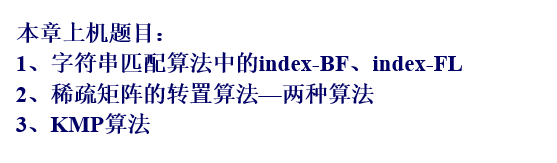
\includegraphics[width=0.7\linewidth]{img/problems}
		\caption*{}
		\label{fig:problem}
	\end{figure}
	
	\section{Code}
	💻💻💻
	\subsection{SMatrix.h}
%	\lstinputlisting[language=c++, 
%	caption={Sparse Matrix header} ,
%	label=SMatrix.h
%	]{src/SMatrix.h}
	
	\begin{longlisting}
		\inputminted{c++}{src/SMatrix.h}
		\caption{Sparse Matrix header}
		\label{SMatrix.h}
	\end{longlisting}
	
	\subsection{SMatrix\_test.cpp}
%	\lstinputlisting[language=c++, 
%	caption={Sparse Matrix test} ,
%	label=SMatrix_test.cpp
%	]{src/SMatrix_test.cpp}	
	
	\begin{longlisting}
		\inputminted{c++}{src/SMatrix_test.cpp}
		\caption{Sparse Matrix test}
		\label{SMatrix_test.cpp}
	\end{longlisting}

	\subsection{mySort.h}
	This is a large file, see it in the \emph{src} folder,
	or view it online \href{
	https://github.com/How-u-doing/DataStructures/blob/master/Sort/mySort.h}
	{here}.
		
		
	\clearpage
	\section{Output}
	\subsection{Win10}
	\begin{figure}[!hb]
		\centering
		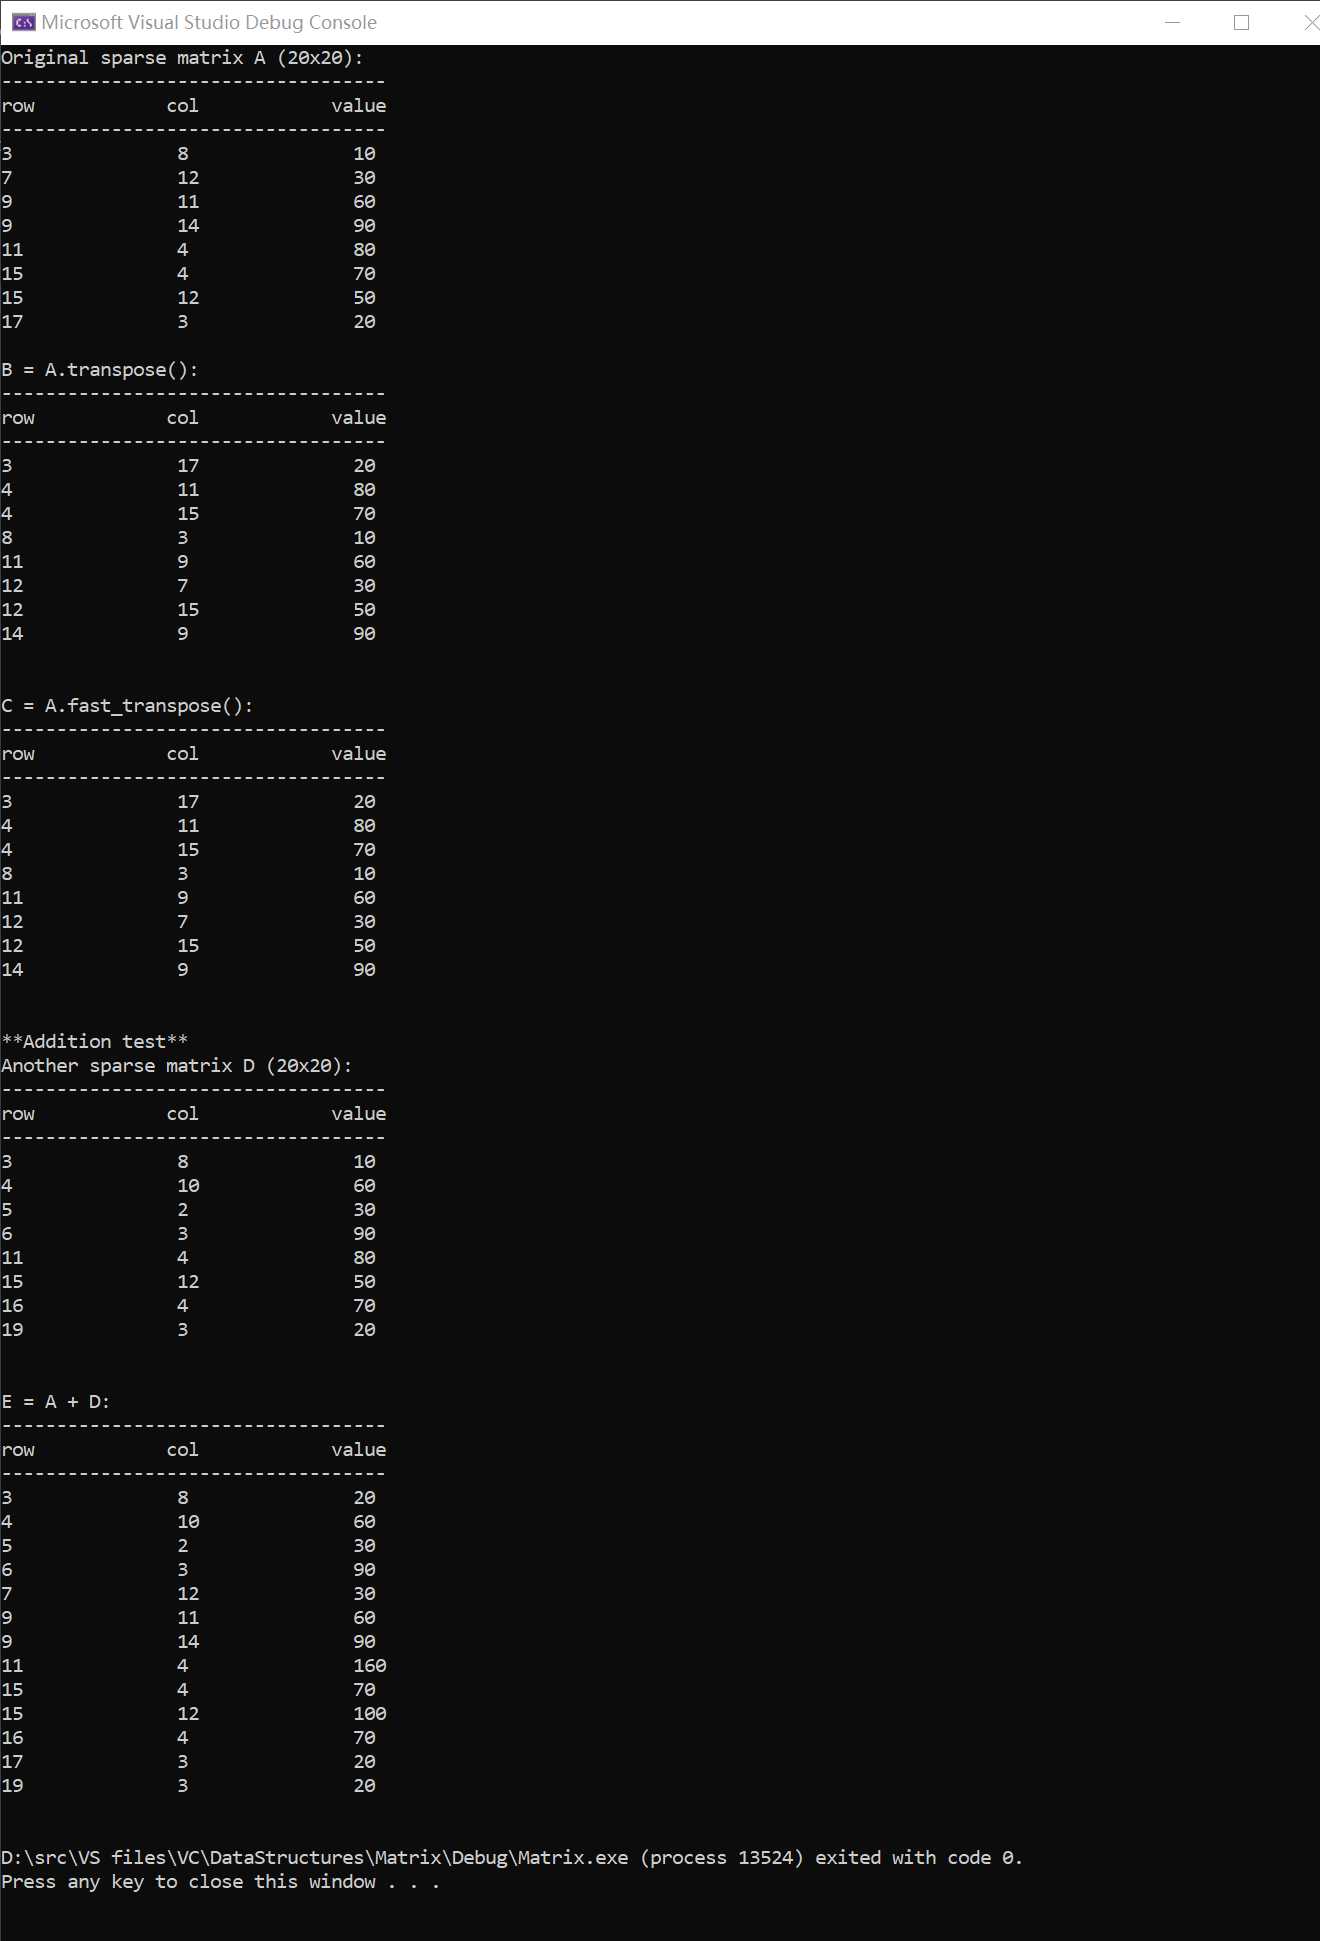
\includegraphics[width=0.75\linewidth]{img/sparse_matrix_tests_win10}
		\caption{Sparse Matrix test results in Win10}
		\label{fig:sparsematrixtestswin10}
	\end{figure}
	
	\clearpage
	\subsection{Linux}
	\begin{figure}[!hb]
		\centering
		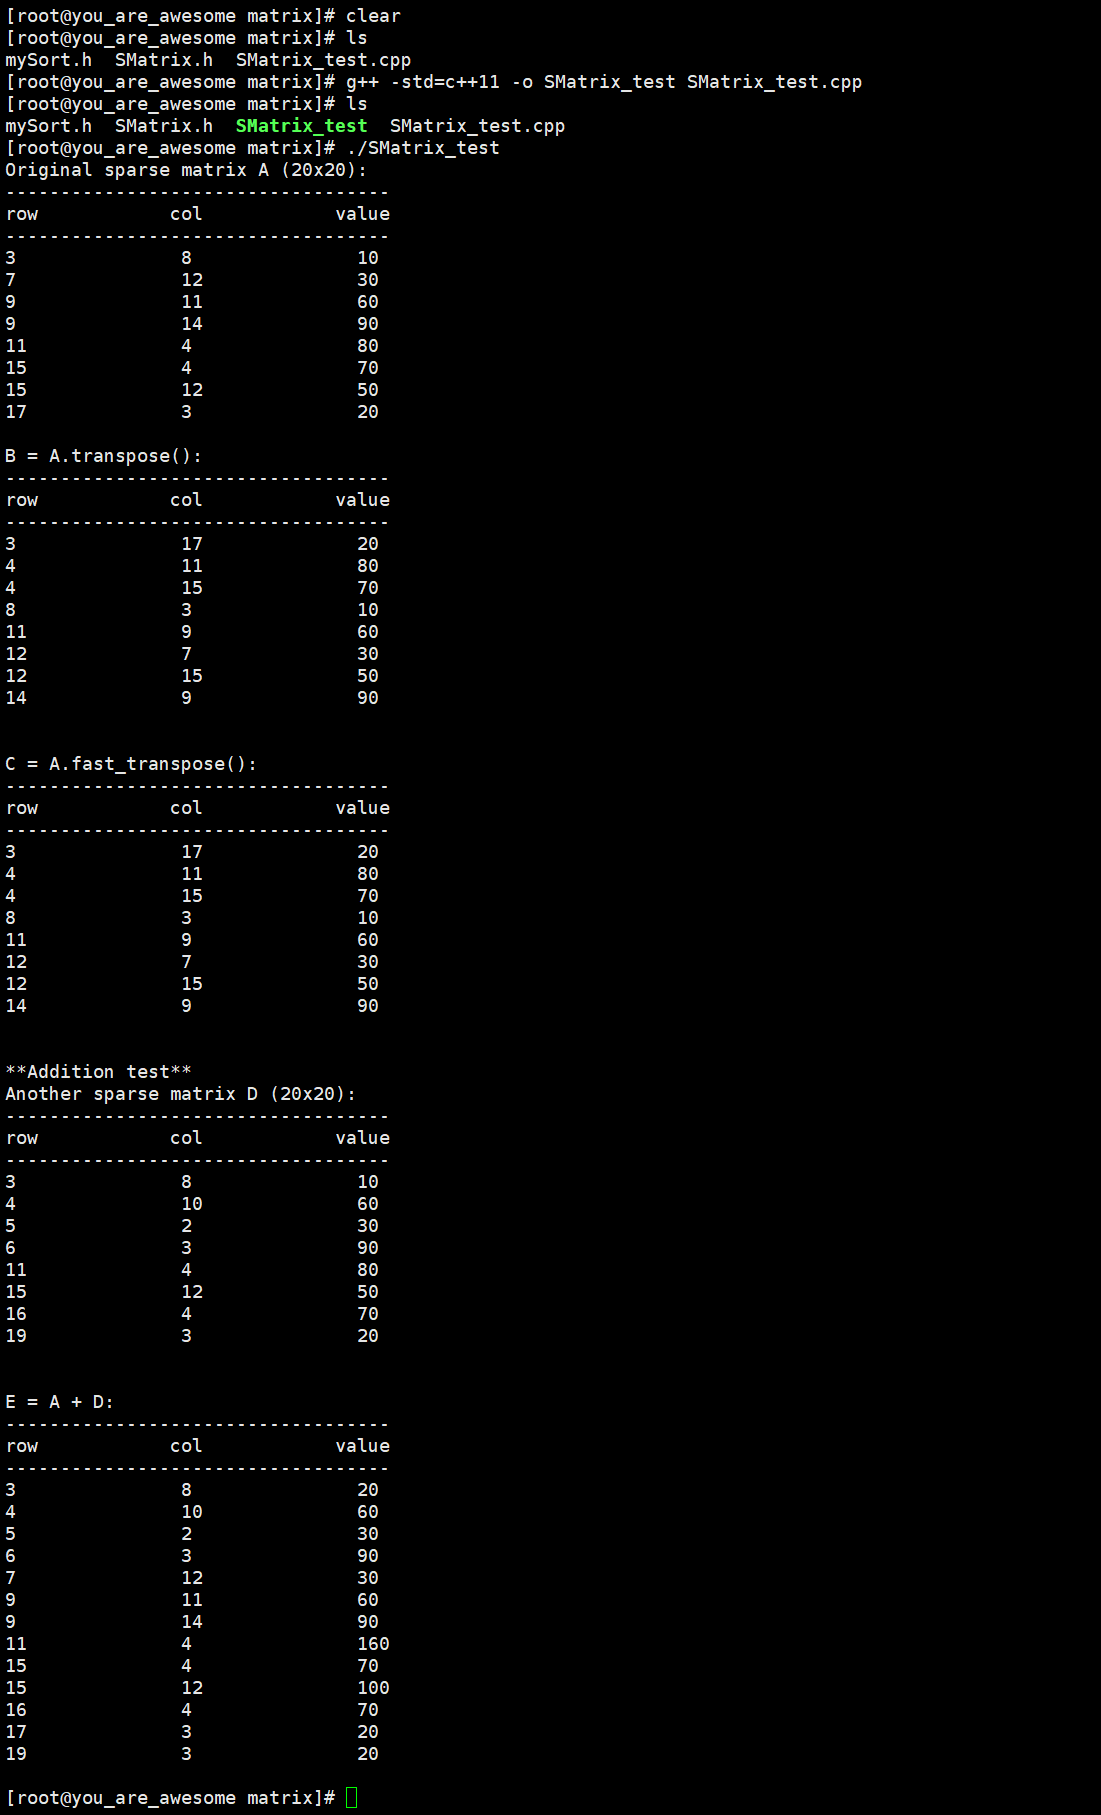
\includegraphics[width=0.75\linewidth]{img/sparse_matrix_tests_centos}
		\caption{Sparse Matrix test results in Linux (CentOS)}
		\label{fig:sparsematrixtestscentos}
	\end{figure}
	

	\section{Appendix}
	\begin{figure}[!hb]
		\centering
		\includegraphics[width=1\linewidth]{\string"img/The 
			Beatles\string".jpg}
		\caption*{Hello from the Beatles.😃}
		\label{fig:the-beatles}
	\end{figure}
	
\end{document}
